\chapter{Complex numbers}
The equation $x^2 + 1 = 0$ has no solution in $\mathbb{R}$. To solve this problem, we introduce a new number $i$ such that $i^2 = -1$.
\begin{proof}
    Let's prove that the equation $x^2 + 1 = 0$ has no solution in $\mathbb{R}$.
    Assume that there exists $x \in \mathbb{R}$ such that $x^2 + 1 = 0$. Then, we have:
    \[
        x^2 = -1
    \]
    However, the left-hand side is non-negative for all $x \in \mathbb{R}$, while the right-hand side is negative. This is a contradiction. Therefore, there are no solutions in $\mathbb{R}$.
\end{proof}

\section{Definition and properties of complex numbers}
\begin{definition}[Complex numbers]
    The set of complex numbers is defined as $\mathbb{C} = \{ a + bi \mid a, b \in \mathbb{R} \}$ where $i$ is the imaginary unit with the property that $i^2 = -1$. Addition and mutliplication of complex numbers are defined as follows:
    \begin{itemize}[itemsep=1pt,label=$\circ$]
        \item $(a + bi) + (c + di) = (a + c) + (b + d)i$
        \item $(a + bi)(c + di) = (ac - bd) + (ad + bc)i$
    \end{itemize}
\end{definition}
Let also add that:
\begin{itemize}[itemsep=1pt,label=$\circ$]
    \item $\exists 0 \in \mathbb{C}: 0 = 0 + 0i$ such as $(a + bi) + (0 + 0i) = (a + bi) \quad \forall a, b \in \mathbb{R}$.
    \item $\exists$ an inverse for $(a + bi): ((-a) + (-b)i) + (a + bi) = 0 + 0i = 0 \quad \forall a, b \in \mathbb{R}$.
    \item $\exists 1 \in \mathbb{C}: 1 = 1 + 0i$ such as $(a + bi)(1 + 0i) = (a + bi) \quad \forall a, b \in \mathbb{R}$.
    \item $\forall z \in \mathbb{C} : z \neq 0 \implies \exists z^{-1} \in \mathbb{C} : z z^{-1} = 1$.
\end{itemize}

\begin{definition}[Inverse of a complex number]
    Let $z = a + bi \in \mathbb{C}$ such as $z \neq 0$ (i.e., $a^2 + b^2 \neq 0$). The inverse of $z$ is given by:
    \[
        z^{-1} = \frac{a}{a^2 + b^2} - \frac{b}{a^2 + b^2}i
    \]
\end{definition}
Let's verify that $z z^{-1} = 1$:
\[
    z z^{-1} = (a + bi) \left( \frac{a}{a^2 + b^2} - \frac{b}{a^2 + b^2}i \right) = \frac{a^2 + b^2}{a^2 + b^2} = 1
\]
\begin{eg}
    Let's verify that complex numbers respect the distributive property. \\ Let $z_1 = (a_1 + b_1 i)$, $z_2 = (a_2 + b_2 i)$ and $z_3 = (a_3 + b_3 i)$ be three complex numbers. We want to show that:
    \[
        z_1(z_2 + z_3) = z_1 z_2 + z_1 z_3
    \]
    Let's compute left side:
    \[
        z_1(z_2 + z_3) = (a_1 + b_1 i)((a_2 + a_3) + (b_2 + b_3)i)
    \]
    \[
        = (a_1(a_2 + a_3) - b_1(b_2 + b_3)) + (a_1(b_2 + b_3) + b_1(a_2 + a_3))i
    \]
    Now, let's compute the right side:
    \[
        z_1 z_2 + z_1 z_3 = (a_1 a_2 - b_1 b_2 + a_1 a_3 - b_1 b_3) + (a_1 b_2 + b_1 a_2 + a_1 b_3 + b_1 a_3)i
    \]
    Both sides are equal, thus $\mathbb{C}$ is a commutative field.
\end{eg}
We can prove that $\mathbb{C}$ is not an ordered field. Indeed, if we assume that $i > 0$, then $i^2 = -1 > 0$ which is a contradiction. If we assume that $i < 0$, then $-i > 0$ and $(-i)^2 = -1 > 0$ which is also a contradiction. Thus, $\mathbb{C}$ is not an ordered field.

\section{Form of complex numbers}
Complex numbers can be represented in 3 different forms.
\subsection{Algebraic form}
\begin{definition}[Algebraic form]
    The algebraic form of a complex number $z = a + bi$ where $a, b \in \mathbb{R}$. Which can also be written as:
    \[
        z = \text{Re}(z) + \text{Im}(z)i
    \]
    where $\text{Re}(z) = a$ is the real part of $z$ and $\text{Im}(z) = b$ is the imaginary part of $z$.
\end{definition}
The modulus of a complex number $z = a + bi$ is defined as:
\[
    |z| = \sqrt{(\text{Re} (z))^2 + (\text{Im} (z))^2} = \sqrt{a^2 + b^2} \geq 0
\]
\[
    |z| = 0 \iff z = 0
\]

\subsection{Trigonometric form}
\begin{definition}[Trigonometric form]
    The trigonometric form of a complex number $z = a + bi$ is given by:
    \[
        z = r(\cos(\theta) + i \sin(\theta)) \quad r \geq 0, \theta \in \mathbb{R}
    \]
    where:
    \begin{center}
        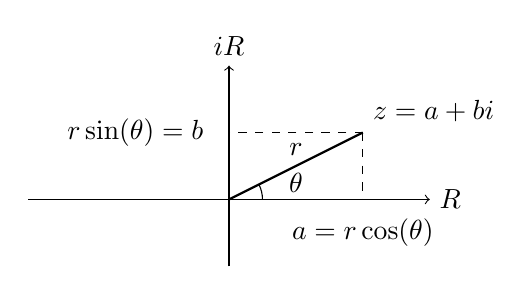
\begin{tikzpicture}[scale=.85]
            \draw[->] (-3,0) -- (3,0) node[right] {$\mathbb{R}$};
            \draw[->] (0,-1) -- (0,2) node[above] {$i \mathbb{R}$};
            \draw[thick] (0,0) -- (2,1) node[above right] {$z = a + bi$};
            \draw[dashed] (2,1) -- (2,0);
            \draw[dashed] (2,1) -- (0,1);
            \draw (0.5,0) arc[start angle=0,end angle=26.57,radius=0.5];
            \node at (1,0.25) {$\theta$};
            \node at (1,.75) {$r$};
            \node at (2,-0.5) {$a = r \cos(\theta)$};
            \node at (-1.4,1) {$r \sin(\theta) = b$};
        \end{tikzpicture}
    \end{center}
    and:
    \[
        \text{Re}(z) = a = r \cos(\theta), \quad \text{Im}(z) = b = r \sin(\theta)
    \]
\end{definition}
$\newline$ %space error
The modulus of $z$ is given by:
\[
    |z| = r = \sqrt{r^2 \cos^2(\theta) + r^2 \sin^2(\theta)} = r \geq 0
\]
The argument of $z$ ($z \neq 0$) is given by:
\[
    r \neq 0 \implies \sin(\theta) = \frac{\text{Im}(z)}{r}, \quad \cos(\theta) = \frac{\text{Re}(z)}{r}
\]
Showing that $\theta$ is defined up to an additive factor of $2k\pi$, $k \in \mathbb{Z}$. Also:
\[
    \tan(\theta) = \frac{\text{Im}(z)}{\text{Re}(z)} = \frac{b}{a} \quad \text{if } a \neq 0
\]
\begin{eg}
    Let's find the argument of $z = a + bi$. We have: \\
    If $a > 0$, then:
    \[
        \theta = \arctan\left(\frac{b}{a}\right) + 2k\pi, \quad k \in \mathbb{Z}
    \]
    \begin{center}
        \begin{tikzpicture}[scale=.85]
            \draw[->] (-3,0) -- (3,0) node[right] {$\mathbb{R}$};
            \draw[->] (0,-1) -- (0,2) node[above] {$i \mathbb{R}$};
            \draw[thick] (0,0) -- (2,1);
            \draw[dashed,color=primary] (2,1) -- (2,0);
            \draw[dashed,color=primary] (2,1) -- (0,1);
            \draw[->,primary] (0.5,0) arc[start angle=0,end angle=26.57,radius=0.5];
            \node[primary] at (2,0.25) {$\theta = \text{arg}(z)$};
            \node[primary] at (2,-0.3) {$a$};
            \node[primary] at (-0.4,1) {$b$};
        \end{tikzpicture}
    \end{center}
    If $a < 0$, then:
    \[
        \theta = \arctan\left(\frac{b}{a}\right) + (2k + 1)\pi, \quad k \in \mathbb{Z}
    \]
    \begin{center}
        \begin{tikzpicture}[scale=.85]
            \draw[->] (-3,0) -- (3,0) node[right] {$\mathbb{R}$};
            \draw[->] (0,-2) -- (0,2) node[above] {$i \mathbb{R}$};

            \draw[thick,secondary] (0,0) -- (2,1);
            \draw[->,secondary] (0.5,0) arc[start angle=0,end angle=25,radius=0.5];
            \node[secondary] at (2.8,0.6) {$\theta \neq \arctan\frac{b}{a}$};

            \draw[thick] (0,0) -- (-2,-1);
            \draw[dashed,primary] (-2,-1) -- (-2,0);
            \draw[dashed,primary] (-2,-1) -- (0,-1);
            \draw[->,primary] (0.7,0) arc[start angle=0,end angle=205,radius=0.7];
            \node[primary] at (-2.3,0.8) {$\arctan\frac{b}{a} + \pi = \theta$};
            \node[primary] at (-2,0.3) {$a$};
            \node[primary] at (0.4,-1) {$b$};
        \end{tikzpicture}
    \end{center}
    Finally, if $a = 0$, then:
    \[
        \theta = \begin{cases}
            \frac{\pi}{2} + 2k\pi, & b > 0 \\
            \frac{3\pi}{2} + 2k\pi, & b < 0 \\
        \end{cases}
    \]
    \begin{center}
        \begin{tikzpicture}[scale=.85]
            \draw[->] (-3,0) -- (3,0) node[right] {$\mathbb{R}$};
            \draw[->] (0,-2) -- (0,2) node[above] {$i \mathbb{R}$};

            \draw[thick,secondary] (0,0) -- (0,1.5);
            \draw[->,secondary] (0.5,0) arc[start angle=0,end angle=90,radius=0.5];
            \node[secondary] at (0.3, 1.5) {$z$};
            \node[secondary] at (1.2,0.5) {$\theta = \frac{\pi}{2}$};

            \draw[thick,primary] (0,0) -- (0,-1.5);
            \draw[->,primary] (0.7,0) arc[start angle=0,end angle=270,radius=0.7];
            \node[primary] at (-0.3, -1.5) {$z$};
            \node[primary] at (-1.5,-0.5) {$\theta = \frac{3\pi}{2}$};
        \end{tikzpicture}
    \end{center}
\end{eg}
$\newline$ %space error
The argument of $z$ is only defined for $z \neq 0$.

\subsection{Exponential form}
\begin{definition}[Exponential form]
    The exponential form of a complex number $z = a + bi$ is given by:
    \[
        e^z = \text{exp}(z) = e^a (\cos(b) + i \sin(b))
    \]
    If $z = a$, then:
    \[
        e^z = e^a (\cos(0) + i \sin(0)) = e^a (1 + 0) = e^a
    \]
    If $z = bi$, then:
    \[
        e^z = e^0 (\cos(b) + i \sin(b)) = e^{ib}
    \]
\end{definition}

\begin{definition}[Euler's formula]
    For any real number $\theta \in \mathbb{R}$, we have:
    \[
        e^{i\theta} = \cos(\theta) + i \sin(\theta)
    \]
\end{definition}
Let's show that $e^{i(\theta_1 + \theta_2)} = e^{i\theta_1} \cdot e^{i\theta_2}$:
\[
    e^{i(\theta_1 + \theta_2)} = \cos(\theta_1 + \theta_2) + i \sin(\theta_1 + \theta_2)
\]
\[
    = (\cos(\theta_1) \cos(\theta_2) - \sin(\theta_1) \sin(\theta_2)) + i (\sin(\theta_1) \cos(\theta_2) + \cos(\theta_1) \sin(\theta_2))
\]
\[
    = (\cos(\theta_1) + i \sin(\theta_1))(\cos(\theta_2) + i \sin(\theta_2)) = e^{i\theta_1} \cdot e^{i\theta_2}
\]
Let's also show that an imaginary exponential is periodic with period $2\pi$:
\[
    y_1 = y_2 + 2k\pi, \ k \in \mathbb{Z} \implies e^{i y_1} = e^{i y_2 + 2k\pi} = e^{i y_2}(\cos(2k\pi) + i \sin(2k\pi)) = e^{i y_2}
\]
If we take a complex number in trigonometric form $z = r(\cos(\theta) + i \sin(\theta))$, we can write it in exponential form as:
\[
    z = r e^{i\theta}
\]

\subsection{Summary of the forms of a complex number}
A complex number can be represented as:
\begin{align*}
    z &= \text{Re}(z) + i \cdot \text{Im}(z) &\text{(Algebraic form)} \\
    &= |z|(\cos(\text{arg}(z)) + i \sin(\text{arg}(z))) &\text{(Trigonometric form)} \\
    &= |z| e^{i \text{arg}(z)} &\text{(Exponential form)} \\
\end{align*}
Usually complex numbers are represented in polar form (trigonometric or exponential form).
\begin{eg}
    Let's show that the modulus of $z = e^{(e^{i \phi})}$ is equal to $e^{\cos(\phi)}$.
    \[
        z = e^{(e^{i \phi})} = e^{(\cos(\phi) + i \sin(\phi))} = e^{\cos(\phi)} e^{i \sin(\phi)} = e^{\cos(\phi)} \cdot (\cos(\sin(\phi)) + i \sin(\sin(\phi)))
    \]
    Thus, the modulus of $z$ is:
    \[
        |z| = \sqrt{(e^{\cos(\phi)})^2 \cdot [(\cos(\sin(\phi)))^2 + (\sin(\sin(\phi)))^2]} = e^{\cos(\phi)}
    \]
\end{eg}

\begin{eg}
    Let's find the exponential form of $z = -1 + i$. We need to calculate the modulus and the argument of $z$:
    \[
        |z| = \sqrt{(-1)^2 + 1^2} = \sqrt{2}
    \]
    Since $\text{Re}(z) = -1 < 0$ and $\text{Im}(z) = 1 > 0$, we are in the second case of the argument calculation:
    \[
        \theta = \arctan\left(\frac{1}{-1}\right) + \pi = -\frac{\pi}{4} + \pi = \frac{3\pi}{4}
    \]
    Thus, the exponential form of $z$ is:
    \[
        z = \sqrt{2} e^{i \frac{3\pi}{4}}
    \]
\end{eg}

\begin{eg}
    Let's find the algebraic form of $z = 5 e^{i \frac{2\pi}{3}}$. We have:
    \[
        z = 5 \left( \cos\left(\frac{2\pi}{3}\right) + i \sin\left(\frac{2\pi}{3}\right) \right) = 5 \left( -\frac{1}{2} + i \frac{\sqrt{3}}{2} \right) = -\frac{5}{2} + i \frac{5\sqrt{3}}{2}
    \]
\end{eg}

\subsection{Operations in polar form}
Polar form is very useful to perform operations on complex numbers.
\begin{definition}[Mutiplication in polar form]
    To multiply two complex numbers in polar form, we multiply their moduli and add their arguments. If $z_1 = r_1 e^{i \theta_1}$ and $z_2 = r_2 e^{i \theta_2}$, then:
    \[
        z_1 z_2 = r_1 r_2 e^{i (\theta_1 + \theta_2)}
    \]
\end{definition}
\begin{proof}
    Let $z_1 = r_1 e^{i \theta_1}$ and $z_2 = r_2 e^{i \theta_2}$. We have:
    \[
        z_1 z_2 = r_1 e^{i \theta_1} \cdot r_2 e^{i \theta_2}
    \]
    By using the property of exponentials, we get:
    \[
        z_1 z_2 = r_1 r_2 e^{i (\theta_1 + \theta_2)}
    \]
\end{proof}

\begin{eg}
    Let $z = e^{i \phi}$, $w = e^{i \psi}$, $|z| = 1$ and $|w| = 1$. Then:
    \[
        z w = e^{i(\phi + \psi)}
    \]
\end{eg}

\begin{definition}[Division in polar form]
    To divide two complex numbers in polar form, we divide their moduli and subtract their arguments. If $z_1 = r_1 e^{i \theta_1}$ and $z_2 = r_2 e^{i \theta_2}$, then:
    \[
        \frac{z_1}{z_2} = \frac{r_1}{r_2} e^{i (\theta_1 - \theta_2)} \quad \text{if } z_2 \neq 0
    \]
\end{definition}

\begin{definition}[Inverse in polar form]
    The inverse of a complex number, $z \neq 0$ in polar form is given by:
    \[
        z^{-1} = \frac{1}{r} e^{-i \theta} \quad \text{if } z = r e^{i \theta} \text{ and } r > 0
    \]
\end{definition}
\begin{proof}
    Let $z = r e^{i \theta}$ such that $r > 0$. We have:
    \[
        z z^{-1} = r e^{i \theta} \cdot \frac{1}{r} e^{-i \theta} = 1 \cdot e^{i(\theta - \theta)} = 1 \cdot e^0 = 1
    \]
\end{proof}

\begin{definition}[De Moivre's theorem]
    For any complex number $z = r e^{i \theta}$ and any integer $n \in \mathbb{N}^*$, we have:
    \[
        z^n = r^n e^{i n \theta} = r^n (\cos(n \theta) + i \sin(n \theta))
    \]
\end{definition}
\begin{proof}
    Let's prove this by induction. For $n = 1$, we have:
    \[
        z^1 = r^1 e^{i \cdot 1 \cdot \theta} = r e^{i \theta}
    \]
    Now, let's assume it's true for $n = k$, i.e., $z^k = r^k e^{i k \theta}$. For $n = k + 1$, we have:
    \[
        z^{k+1} = z^k z = (r^k e^{i k \theta})(r e^{i \theta}) = r^k r e^{i k \theta} e^{i \theta} = r^{k+1} e^{i (k+1) \theta}
    \]
    Thus, by induction, the theorem holds for all $n \in \mathbb{N}^*$.
\end{proof}

\subsection{The Most Beautiful Formula in Mathematics}
Let $y = \pi$, then:
\[e^{i\pi} = \cos(\pi) + i \sin(\pi) = -1 + 0 = -1\]
\begin{theorem}[Euler's identity]
    \[e^{i\pi} + 1 = 0
    \]
\end{theorem}
This formula links the 5 most important constants in mathematics: $e, i, \pi, 1, 0$.

\section{Conjugate of a complex number}
\begin{definition}[Conjugate of a complex number]
    The conjugate of a complex number $z = a + bi$ is defined as:
    \[
        \overline{z} = a - bi
    \]
    or in polar form for $z = r e^{i \theta}$:
    \[
        \overline{z} = r e^{-i \theta} = r(\cos(-\theta) + i \sin(-\theta)) = r(\cos(\theta) - i \sin(\theta))
    \]
\end{definition}
If $\bar{z} \neq 0$, then:
\[
    z \bar{z} = (a + bi)(a - bi) = a^2 + b^2 = |z|^2
\]

\subsection{Properties of the conjugate}
Let $z_1, z_2 \in \mathbb{C}$ and $\lambda \in \mathbb{R}$, we have:
\begin{itemize}[itemsep=1pt,label=$\circ$]
    \item $\overline{\overline{z}} = z$
    \item $\overline{z_1 \pm z_2} = \overline{z_1} \pm \overline{z_2}$
    \item $\overline{z_1 z_2} = \overline{z_1} \, \overline{z_2}$
    \item $\overline{\left(\frac{z_1}{z_2}\right)} = \frac{\overline{z_1}}{\overline{z_2}}$ if $z_2 \neq 0$
    \item $\overline{\lambda z} = \lambda \overline{z}$
\end{itemize}
Also, we have:
\begin{itemize}[itemsep=1pt,label=$\circ$]
    \item $\text{Re}(z) = \frac{z + \overline{z}}{2}$
    \item $\text{Im}(z) = \frac{z - \overline{z}}{2i}$
\end{itemize}
If $|z| = 1$, then in polar form for $z = \cos(\phi) + i \sin(\phi)$, we have:
\[
    \cos(\phi) = \frac{e^{i\phi} + e^{-i\phi}}{2}, \quad \sin(\phi) = \frac{e^{i\phi} - e^{-i\phi}}{2i}
\]

\begin{eg}
    Let's express $(\sin(\phi))^4$:
    \[
        (\sin(\phi))^4 = \left( \frac{e^{i\phi} - e^{-i\phi}}{2i} \right)^4 = \frac{(e^{i\phi} - e^{-i\phi})^4}{16 i^4} = \frac{e^{4i\phi} - 4e^{2i\phi} + 6 - 4e^{-2i\phi} + e^{-4i\phi}}{16}
    \]
    Since $-4e^{2i\phi} - 4e^{-2i\phi} = -8 \cos(2\phi)$ and $e^{4i\phi} + e^{-4i\phi} = 2 \cos(4\phi)$, we get:
    \[
        (\sin(\phi))^4 = \frac{3}{8} - \frac{1}{2} \cos(2\phi) + \frac{1}{8} \cos(4\phi)
    \]
\end{eg}

\section{Roots of complex numbers}
\begin{definition}[n-th roots of a complex number]
    Let $z \in \mathbb{C}^*$ and $n \in \mathbb{N}^*$. The n-th roots of $z$ are the solutions of the equation:
    \[    w^n = z
    \]
    If we write $z$ in polar form as $z = r e^{i \theta}$, then the n-th roots of $z$ are given by:
    \[
        w_k = r^{\frac{1}{n}} e^{i \frac{\theta + 2k\pi}{n}} \quad k = 0, 1, \ldots, n-1
    \]
    There are $n$ distinct n-th roots of $z$.
\end{definition}
\begin{proof}
    Let $w = \rho e^{i \phi}$ be an n-th root of $z$. We have:
    \[
        w^n = (\rho e^{i \phi})^n = \rho^n e^{i n \phi} = r e^{i \theta}
    \]
    By comparing the moduli and arguments, we get:
    \[
        \rho^n = r \implies \rho = r^{\frac{1}{n}}
    \]
    and
    \[
        n \phi = \theta + 2k\pi \implies \phi = \frac{\theta + 2k\pi}{n} \quad k \in \mathbb{Z}
    \]
    Since the argument is defined up to an additive factor of $2\pi$, we only need to consider $k = 0, 1, \ldots, n-1$ to get all distinct n-th roots. Thus, the n-th roots of $z$ are given by:
    \[
        w_k = r^{\frac{1}{n}} e^{i \frac{\theta + 2k\pi}{n}} \quad k = 0, 1, \ldots, n-1
    \]
\end{proof}

\begin{eg}
    Let $z^2 = w = re^{i \theta}$ (where $r > 0$) be a complex number. Then:
    \[
        z_k = r^{\frac{1}{2}} e^{i \frac{\theta + 2k\pi}{2}} \quad k = 0, 1
    \]
    Thus, the two square roots of $w$ are:
    \[        z_0 = r^{\frac{1}{2}} e^{i \frac{\theta}{2}}, \quad z_1 = r^{\frac{1}{2}} e^{i \left(\frac{\theta}{2} + \pi\right)} = -r^{\frac{1}{2}} e^{i \frac{\theta}{2}} = -z_0
    \]
    More explicitly:
    \[
        (z_1)^2 = (z_2)^2 = w
    \]
\end{eg}

\begin{eg}
    Let's solve the equation $z^3 = -1 + i$ ($z \in \mathbb{C})$. Let $w = -1 + i = \sqrt{2} e^{i \frac{3\pi}{4}}$ be the complex number. We have:
    \[
        z_k = (\sqrt{2})^{\frac{1}{3}} e^{i \frac{\frac{3\pi}{4} + 2k\pi}{3}} = 2^{\frac{1}{6}} e^{i \left(\frac{\pi}{4} + \frac{2k\pi}{3}\right)} \quad k = 0, 1, 2
    \]
    Thus, the three cube roots of $w$ are:
    \[
        z_0 = 2^{\frac{1}{6}} e^{i \frac{\pi}{4}}, \quad z_1 = 2^{\frac{1}{6}} e^{i \left(\frac{\pi}{4} + \frac{2\pi}{3}\right)} = 2^{\frac{1}{6}} e^{i \frac{11\pi}{12}}, \quad z_2 = 2^{\frac{1}{6}} e^{i \left(\frac{\pi}{4} + \frac{4\pi}{3}\right)} = 2^{\frac{1}{6}} e^{i \frac{19\pi}{12}}
    \]
\end{eg}

\begin{eg}
    Let $z \in \mathbb{C}, z \neq 0$. We want to find all complex numbers such that $(\frac{z}{\bar{z}})^3 = \bar{z}$. We have:
    \[
        z = r e^{i \theta} \implies \bar{z} = r e^{-i \theta}
    \]
    Thus:
    \[
        \left(\frac{z}{\bar{z}}\right)^3 = \left(\frac{r e^{i \theta}}{r e^{-i \theta}}\right)^3 = (e^{2i \theta})^3 = e^{6i \theta}
    \]
    We want to solve:
    \[        e^{6i \theta} = r e^{-i \theta}
    \]
    By comparing the moduli and arguments, we get:
    \[        r = 1
    \]
    and
    \[        6 \theta = -\theta + 2k\pi \implies 7 \theta = 2k\pi \implies \theta = \frac{2k\pi}{7}, \quad k \in \mathbb{Z}
    \]
    Thus, the solutions are:
    \[        z_k = e^{i \frac{2k\pi}{7}}, \quad k = 0, 1, \ldots, 6 \]
\end{eg}

\section{Polynomials with complex coefficients}
\begin{definition}[Polynomial with complex coefficients]
    A polynomial with complex coefficients is a function $P: \mathbb{C} \to \mathbb{C}$ defined by:
    \[
        P(z) = a_n z^n + a_{n-1} z^{n-1} + \ldots + a_1 z + a_0
    \]
    where $a_0, a_1, \ldots, a_n \in \mathbb{C}$ and $a_n \neq 0$. The degree of the polynomial is $n$.
\end{definition}
In the case of quadratic polynomials, like in the case with real coefficients, we have:
\[
    z = \frac{-b \pm \sqrt{b^2 - 4ac}}{2a}
\]
except that now $a, b, c \in \mathbb{C}$, thus:
\[
    \sqrt{b^2 - 4ac} \in \mathbb{C} \implies w \in \mathbb{C} : w^2 = b^2 - 4ac
\]

\begin{theorem}[Fundamental Theorem of Algebra]
    Every non-constant polynomial with complex coefficients, $P(z) = a_n z^n + a_{n-1} z^{n-1} + \ldots + a_1 z + a_0$ where $a_n \neq 0$ can be factored as:
    \[
        P(z) = a_n (z - z_1)^{m_1}(z - z_2)^{m_2} \ldots (z - z_n)^{m_n}
    \]
    where $z_1, z_2, \ldots, z_n \in \mathbb{C}$ are the distinct roots of $P(z)$ and $m_1, m_2, \ldots, m_n \in \mathbb{N}^*$ ($m_1 + m_2 + \ldots + m_n = n$) are their respective multiplicities.
\end{theorem}

\begin{eg}
    Let's check if $P(z) = z^2 + (1-i)z - i$ is divisible by $z - i$. We have:
    \[        P(i) = i^2 + (1-i)i - i = -1 + i + 1 - i = 0
    \]
    Thus, $P(z)$ is divisible by $z - i$.
\end{eg}

\subsection{Polynomials with real coefficients}
If $P(x) = a_n x^n + a_{n-1} x^{n-1} + \ldots + a_1 x + a_0$ is a polynomial with real coefficients, then its complex roots come in conjugate pairs. That is, if $z = a + bi$ is a root of $P(x)$, then its conjugate $\bar{z} = a - bi$ is also a root of $P(x)$.
\begin{proof}
    Let $z = a + bi$ be a root of $P(x)$, then:
    \[        P(z) = a_n z^n + a_{n-1} z^{n-1} + \ldots + a_1 z + a_0 = 0
    \]
    Taking the complex conjugate of both sides, we get:
    \[        \overline{P(z)} = \overline{a_n z^n + a_{n-1} z^{n-1} + \ldots + a_1 z + a_0} = 0
    \]
    Since the coefficients are real, this simplifies to:
    \[        P(\bar{z}) = a_n \bar{z}^n + a_{n-1} \bar{z}^{n-1} + \ldots + a_1 \bar{z} + a_0 = 0
    \]
    Thus, $\bar{z}$ is also a root of $P(x)$.
\end{proof}
Every polynomial with real coefficients of degree $n \geq 2$ can be factored as a product of linear and irreducible quadratic factors with real coefficients.

\section{Subset of complex numbers}
\begin{eg}
    Let $z_o \in \mathbb{C}, r \in \mathbb{R} > 0$. The set of complex numbers defined by:
    \[        |z - z_0| = r
    \]
    where $z = x + yi$ and $z_0 = x_0 + y_0 i$, can be expressed as:
    \[        |(x + yi) - (x_0 + y_0 i)| = r
    \]
    \[        \sqrt{(x - x_0)^2 + (y - y_0)^2} = r
    \]
    \[        (x - x_0)^2 + (y - y_0)^2 = r^2
    \]
    This is the equation of a circle with center $(x_0, y_0)$ and radius $r$ in the Cartesian plane. Thus, the set of complex numbers $z$ such that $|z - z_0| = r$ represents a circle in the complex plane with center $z_0$ and radius $r$.
\end{eg}

\begin{eg}
    Let $z \in \mathbb{C}^*: (\frac{|z|}{z})^4 = \frac{1}{\sqrt{2}}(1 + i)$. We have:
    \[        z = r e^{i \theta} \implies |z| = r, \quad \frac{|z|}{z} = \frac{r}{r e^{i \theta}} = e^{-i \theta}
    \]
    Thus:
    \[        (e^{-i \theta})^4 = e^{-4i \theta} = \frac{1}{\sqrt{2}}(1 + i) = e^{i \frac{\pi}{4}}
    \]
    By comparing the arguments, we get:
    \[        -4 \theta = \frac{\pi}{4} + 2k\pi \implies \theta = -\frac{\pi}{16} - \frac{k\pi}{2}, \quad k = 0,1,2,3
    \]
    Thus, the solutions are:
    \[        \theta \in \left\{ -\frac{\pi}{16} - \frac{k\pi}{2} \mid k = 0,1,2,3 \right\}
    \]
    and $r$ can take any positive real value. Therefore, the geometric representation of the solutions is given by 4 open half-lines originating from the origin, making angles of $-\frac{\pi}{16}, -\frac{9\pi}{16}, -\frac{17\pi}{16}, -\frac{25\pi}{16}$ with the positive real axis.
\end{eg}

\section{Exercices} % week 3 assignement
This section gathers a selection of exercises related to Chapter \thechapter, taken from weekly assignments, past exams, textbooks, and other sources. The origin of each exercise will be indicated at its beginning.